% SPDX-FileCopyrightText: 2026 Cyprien PIERRE
% SPDX-License-Identifier: CC-BY-4.0
\documentclass[tikz,border=5pt]{standalone}
\usepackage[T1]{fontenc}
\usepackage{lmodern}
\usepackage{amsmath,amssymb}
\usetikzlibrary{arrows.meta,positioning}
\begin{document}
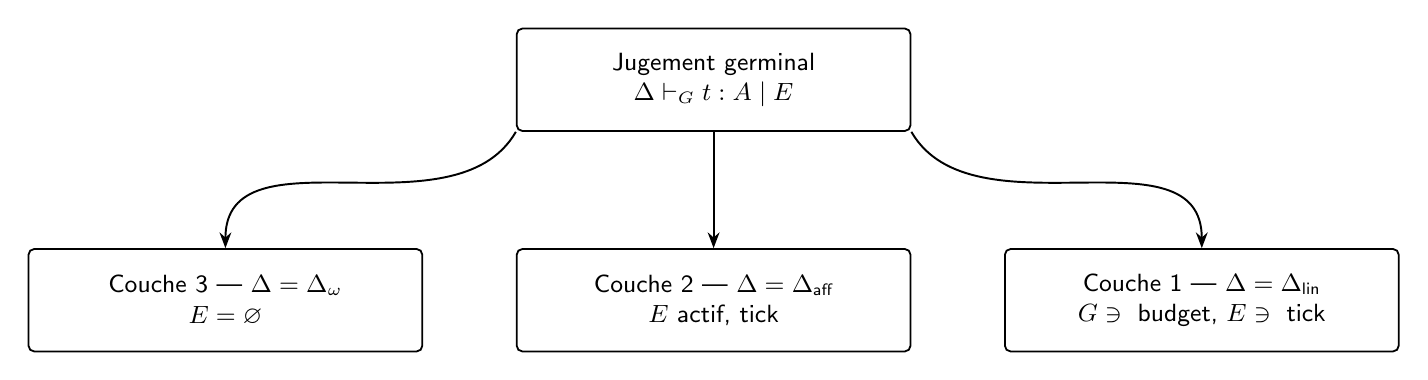
\begin{tikzpicture}[
  font=\sffamily\small,
  box/.style={draw, rounded corners=2pt, align=center, line width=.65pt, minimum height=13mm, minimum width=50mm},
  arrow/.style={-{Stealth[length=2mm]}, line width=.7pt}
]
\node[box] (germ) at (0,0) {Jugement germinal\\$\Delta \vdash_{G} t : A \mid E$};
\node[box] (l3) at (-62mm,-28mm) {Couche 3 --- $\Delta = \Delta_{\omega}$\\$E = \varnothing$};
\node[box] (l2) at (0,-28mm) {Couche 2 --- $\Delta = \Delta_{\text{aff}}$\\$E$ actif, tick};
\node[box] (l1) at (62mm,-28mm) {Couche 1 --- $\Delta = \Delta_{\text{lin}}$\\$G \ni{}$ budget, $E \ni{}$ tick};
\draw[arrow] (germ.south west) to[out=-120, in=90] (l3.north);
\draw[arrow] (germ) -- (l2);
\draw[arrow] (germ.south east) to[out=-60, in=90] (l1.north);
\end{tikzpicture}
\end{document}
